\documentclass[ignorenonframetext,]{beamer}
\setbeamertemplate{caption}[numbered]
\setbeamertemplate{caption label separator}{: }
\setbeamercolor{caption name}{fg=normal text.fg}
\beamertemplatenavigationsymbolsempty
\usepackage{lmodern}
\usepackage{amssymb,amsmath}
\usepackage{ifxetex,ifluatex}
\usepackage{fixltx2e} % provides \textsubscript
\ifnum 0\ifxetex 1\fi\ifluatex 1\fi=0 % if pdftex
  \usepackage[T1]{fontenc}
  \usepackage[utf8]{inputenc}
\else % if luatex or xelatex
  \ifxetex
    \usepackage{mathspec}
  \else
    \usepackage{fontspec}
  \fi
  \defaultfontfeatures{Ligatures=TeX,Scale=MatchLowercase}
\fi
\usetheme[]{AnnArbor}
\usecolortheme{dolphin}
\usefonttheme{structuresmallcapsserif}
% use upquote if available, for straight quotes in verbatim environments
\IfFileExists{upquote.sty}{\usepackage{upquote}}{}
% use microtype if available
\IfFileExists{microtype.sty}{%
\usepackage{microtype}
\UseMicrotypeSet[protrusion]{basicmath} % disable protrusion for tt fonts
}{}
\newif\ifbibliography
\hypersetup{
            pdftitle={SOO and Matching},
            pdfauthor={Annie Chen},
            pdfborder={0 0 0},
            breaklinks=true}
\urlstyle{same}  % don't use monospace font for urls
\usepackage{color}
\usepackage{fancyvrb}
\newcommand{\VerbBar}{|}
\newcommand{\VERB}{\Verb[commandchars=\\\{\}]}
\DefineVerbatimEnvironment{Highlighting}{Verbatim}{commandchars=\\\{\}}
% Add ',fontsize=\small' for more characters per line
\usepackage{framed}
\definecolor{shadecolor}{RGB}{248,248,248}
\newenvironment{Shaded}{\begin{snugshade}}{\end{snugshade}}
\newcommand{\KeywordTok}[1]{\textcolor[rgb]{0.13,0.29,0.53}{\textbf{#1}}}
\newcommand{\DataTypeTok}[1]{\textcolor[rgb]{0.13,0.29,0.53}{#1}}
\newcommand{\DecValTok}[1]{\textcolor[rgb]{0.00,0.00,0.81}{#1}}
\newcommand{\BaseNTok}[1]{\textcolor[rgb]{0.00,0.00,0.81}{#1}}
\newcommand{\FloatTok}[1]{\textcolor[rgb]{0.00,0.00,0.81}{#1}}
\newcommand{\ConstantTok}[1]{\textcolor[rgb]{0.00,0.00,0.00}{#1}}
\newcommand{\CharTok}[1]{\textcolor[rgb]{0.31,0.60,0.02}{#1}}
\newcommand{\SpecialCharTok}[1]{\textcolor[rgb]{0.00,0.00,0.00}{#1}}
\newcommand{\StringTok}[1]{\textcolor[rgb]{0.31,0.60,0.02}{#1}}
\newcommand{\VerbatimStringTok}[1]{\textcolor[rgb]{0.31,0.60,0.02}{#1}}
\newcommand{\SpecialStringTok}[1]{\textcolor[rgb]{0.31,0.60,0.02}{#1}}
\newcommand{\ImportTok}[1]{#1}
\newcommand{\CommentTok}[1]{\textcolor[rgb]{0.56,0.35,0.01}{\textit{#1}}}
\newcommand{\DocumentationTok}[1]{\textcolor[rgb]{0.56,0.35,0.01}{\textbf{\textit{#1}}}}
\newcommand{\AnnotationTok}[1]{\textcolor[rgb]{0.56,0.35,0.01}{\textbf{\textit{#1}}}}
\newcommand{\CommentVarTok}[1]{\textcolor[rgb]{0.56,0.35,0.01}{\textbf{\textit{#1}}}}
\newcommand{\OtherTok}[1]{\textcolor[rgb]{0.56,0.35,0.01}{#1}}
\newcommand{\FunctionTok}[1]{\textcolor[rgb]{0.00,0.00,0.00}{#1}}
\newcommand{\VariableTok}[1]{\textcolor[rgb]{0.00,0.00,0.00}{#1}}
\newcommand{\ControlFlowTok}[1]{\textcolor[rgb]{0.13,0.29,0.53}{\textbf{#1}}}
\newcommand{\OperatorTok}[1]{\textcolor[rgb]{0.81,0.36,0.00}{\textbf{#1}}}
\newcommand{\BuiltInTok}[1]{#1}
\newcommand{\ExtensionTok}[1]{#1}
\newcommand{\PreprocessorTok}[1]{\textcolor[rgb]{0.56,0.35,0.01}{\textit{#1}}}
\newcommand{\AttributeTok}[1]{\textcolor[rgb]{0.77,0.63,0.00}{#1}}
\newcommand{\RegionMarkerTok}[1]{#1}
\newcommand{\InformationTok}[1]{\textcolor[rgb]{0.56,0.35,0.01}{\textbf{\textit{#1}}}}
\newcommand{\WarningTok}[1]{\textcolor[rgb]{0.56,0.35,0.01}{\textbf{\textit{#1}}}}
\newcommand{\AlertTok}[1]{\textcolor[rgb]{0.94,0.16,0.16}{#1}}
\newcommand{\ErrorTok}[1]{\textcolor[rgb]{0.64,0.00,0.00}{\textbf{#1}}}
\newcommand{\NormalTok}[1]{#1}

% Prevent slide breaks in the middle of a paragraph:
\widowpenalties 1 10000
\raggedbottom

\AtBeginPart{
  \let\insertpartnumber\relax
  \let\partname\relax
  \frame{\partpage}
}
\AtBeginSection{
  \ifbibliography
  \else
    \let\insertsectionnumber\relax
    \let\sectionname\relax
    \frame{\sectionpage}
  \fi
}
\AtBeginSubsection{
  \let\insertsubsectionnumber\relax
  \let\subsectionname\relax
  \frame{\subsectionpage}
}

\setlength{\parindent}{0pt}
\setlength{\parskip}{6pt plus 2pt minus 1pt}
\setlength{\emergencystretch}{3em}  % prevent overfull lines
\providecommand{\tightlist}{%
  \setlength{\itemsep}{0pt}\setlength{\parskip}{0pt}}
\setcounter{secnumdepth}{0}
\usepackage{multirow}
\usepackage{graphicx}
\graphicspath{ {./images/} }
\newcommand{\indep}{\rotatebox[origin=c]{90}{$\models$}}

\title{SOO and Matching}
\author{Annie Chen}
\date{Jan. 29, 2020}

\begin{document}
\frame{\titlepage}

\begin{frame}{Review}

\(ATT = \mathbb{E}[Y_{i}(1) - Y_{i}(0) | D_i = 1]\)

\begin{itemize}
\tightlist
\item
  \color{red}{Is this identified when D is not randomized?}
\item
  \color{blue}{Fundamental Problem of Causal Inference}
\end{itemize}

Under what assumptions can the ATE and ATT be non-parametrically
identified?

\begin{itemize}
\item
  \(\{ Y_{i}(0), Y_{i}(1) \} \indep \ D_i \mid X_i = x\) for all
  \(x \in \mathcal{X}\)
\item
  \(0 < \Pr(D_i = 1 \mid X_i = x) < 1\) for all \(x \in \mathcal{X}\)
\end{itemize}

\end{frame}

\begin{frame}{Identification of ATT under CI and Common Support}

\(\tau_{ATT} = \mathbb{E}[Y_{i}(1) - Y_{i}(0) | D_i = 1]\)

\begin{itemize}
\item
  \(= \int \mathbb{E}[Y_{i}(1) - Y_{i}(0) | X_i=x, D_i = 1] f(x|D_i=1)dx\)
  \color{blue}{by law of iterated expectation}\footnote<.->{Recall:
    \(\mathbb{E}[Y] = \mathbb{E}[\mathbb{E}[Y|X]]\) and
    \(\mathbb{E}[X] = \int xf(x)dx\) (continuous)}
\item
  \(= \int \{\mathbb{E}[Y_{i}(1) | X_i=x, D_i = 1] - \mathbb{E}[Y_{i}(0) | X_i=x, D_i = 1]\} f(x|D_i=1)dx\)
  \color{blue}{linearity of expectation}
\item
  \(= \int \mathbb{E}[Y_{i} | X_i=x, D_i = 1] - \mathbb{E}[Y_{i} | X_i=x, D_i = 0] f(x|D_i=1)dx\)\footnote<.->{Turns
    out, ATT is identifiable under a weaker set of assumptions. Compare
    overlap and ignorability assumptions required for identification in
    ATE v. ATT.}
\end{itemize}

Similarly, \(\tau_{ATE} = \mathbb{E}[Y_{i}(1) - Y_{i}(0)]\)

\begin{itemize}
\item
  \(= \int \mathbb{E}[Y_{i}(1) - Y_{i}(0) | X_i=x] f(x)dx\)
\item
  \(= \int (\mathbb{E}[Y_i | X_i=x, D_i = 1] - \mathbb{E}[Y_i | X_i=x, D_i = 0]) f(x)dx\)
\end{itemize}

\end{frame}

\begin{frame}[fragile]{\texttt{Matching} package}

The workhorse of the package:

\begin{itemize}
\item
  \texttt{Match(Y,\ Tr,\ X,\ estimand\ =\ "ATT",\ M\ =\ 1,\ exact,\ Weight...)}

  \begin{itemize}
  \item
    By default, the function estimates the ATT, \texttt{exact\ =\ NULL},
    \texttt{replace\ =\ TRUE}, and uses one-to-one matching
    (\texttt{M\ =\ 1}).
  \item
    Other arguments: (\texttt{ties}, \texttt{caliper},
    \texttt{BiasAdjust}, \texttt{CommonSupport})
  \item
    \texttt{Weight} = 2 (Mahalanobis distance), 3 (custom supplied by
    \texttt{Weight.matric})
  \item
    use \texttt{summary()} on matched object
  \end{itemize}
\end{itemize}

\end{frame}

\begin{frame}[fragile]{\texttt{Matching} package}

Check the balance before and after matching using these functions to
create tables:

\begin{itemize}
\item
  \texttt{MatchBalance(formula,\ data,\ match.out...)}
\item
  \texttt{baltest.collect(matchbal.out,\ var.names)}
\end{itemize}

\end{frame}

\begin{frame}[fragile]{Alternatively, the \texttt{MatchIt} package}

\begin{itemize}
\item
  \texttt{matchit(formula,\ data,\ method\ =\ "nearest",\ discard\ =\ "none",\ distance\ =\ "logit")}
\item
  \texttt{method} =
  \texttt{{[}"genetic",\ "exact",\ "subclass",\ "nearest",\ ...{]}}
\item
  I.e. \texttt{nearest} selects the \(r\) (default = 1) best control
  matches for each individual in the treatment group (excluding
  discarded).
\end{itemize}

\end{frame}

\begin{frame}[fragile]{Job Training Example (Lalonde 1986)}

\begin{Shaded}
\begin{Highlighting}[]
\KeywordTok{data}\NormalTok{(lalonde)}
\end{Highlighting}
\end{Shaded}

This is a subsample of the original data consisting of the National
Supported Work Demonstration (NSW) treated group and the comparison
sample from the Population Survey of Income Dynamics (PSID).
(non-experimental study)

\begin{itemize}
\tightlist
\item
  \texttt{treat}: participation in the job training program
\item
  \texttt{re78}: 1978 real earnings
\end{itemize}

\end{frame}

\begin{frame}[fragile]{Job Training Example (Lalonde 1986)}

A naive comparison of earnings for those who participated and those who
did not.

\small

\begin{Shaded}
\begin{Highlighting}[]
\NormalTok{lalonde }\OperatorTok\StringTok{ }\KeywordTok{group_by}\NormalTok{(treat) }\OperatorTok
\StringTok{   }\KeywordTok{summarise}\NormalTok{(}\DataTypeTok{Income1978 =} \KeywordTok{mean}\NormalTok{(re78), }\DataTypeTok{n =} \KeywordTok{n}\NormalTok{())}
\end{Highlighting}
\end{Shaded}

\begin{verbatim}
## # A tibble: 2 x 3
##   treat Income1978     n
##   <int>      <dbl> <int>
## 1     0      6984.   429
## 2     1      6349.   185
\end{verbatim}

\normalsize

\end{frame}

\begin{frame}[fragile]

\small
Specify pre-treatment covariates to match on.

\begin{Shaded}
\begin{Highlighting}[]
\NormalTok{bal_form <-}\StringTok{ }\KeywordTok{formula}\NormalTok{(treat }\OperatorTok{~}\StringTok{ }\NormalTok{age }\OperatorTok{+}\StringTok{ }\NormalTok{educ }\OperatorTok{+}\StringTok{ }\NormalTok{black }\OperatorTok{+}\StringTok{ }\NormalTok{hispan }\OperatorTok{+}\StringTok{ }
\StringTok{                      }\NormalTok{nodegree }\OperatorTok{+}\StringTok{ }\NormalTok{married }\OperatorTok{+}\StringTok{ }\NormalTok{re74 }\OperatorTok{+}\StringTok{ }\NormalTok{re75 }\OperatorTok{+}\StringTok{ }\NormalTok{re78)}
\CommentTok{# or}
\CommentTok{# as.formula(paste("treat~",paste(names(lalonde)[-1],collapse="+")))}
\end{Highlighting}
\end{Shaded}

\normalsize

Let's check the pre-matching balance.

\small

\begin{Shaded}
\begin{Highlighting}[]
\NormalTok{mb_unmatched <-}\StringTok{ }\KeywordTok{MatchBalance}\NormalTok{(bal_form, }
                             \DataTypeTok{data =}\NormalTok{ lalonde, }\DataTypeTok{print.level=}\DecValTok{0}\NormalTok{)}
\NormalTok{tab_unmatched <-}\StringTok{ }\KeywordTok{baltest.collect}\NormalTok{(mb_unmatched, }
                                 \DataTypeTok{var.names =} \KeywordTok{colnames}\NormalTok{(lalonde)[}\OperatorTok{-}\DecValTok{1}\NormalTok{], }
                                 \DataTypeTok{after =} \OtherTok{FALSE}\NormalTok{)}
\end{Highlighting}
\end{Shaded}

\normalsize

\end{frame}

\begin{frame}

\begin{table}[ht]
\centering
\caption{Covariate Balance in Unmatched Data} 
\label{tab:unmatched-bal}
\scalebox{0.80}{
\begin{tabular}{rrrrrrrr}
  \hline
 & mean.Tr & mean.Co & sdiff & sdiff.pooled & var.ratio & T pval & KS pval \\ 
  \hline
age & 25.82 & 28.03 & -30.94 & -24.19 & 0.44 & 0.00 & 0.00 \\ 
  educ & 10.35 & 10.24 & 5.50 & 4.48 & 0.50 & 0.58 & 0.02 \\ 
  black & 0.84 & 0.20 & 175.68 & 166.77 & 0.82 & 0.00 &  \\ 
  hispan & 0.06 & 0.14 & -34.89 & -27.69 & 0.46 & 0.00 &  \\ 
  married & 0.71 & 0.60 & 24.43 & 23.50 & 0.86 & 0.01 &  \\ 
  nodegree & 0.19 & 0.51 & -82.41 & -71.95 & 0.62 & 0.00 &  \\ 
  re74 & 2095.57 & 5619.24 & -72.11 & -59.58 & 0.52 & 0.00 & 0.00 \\ 
  re75 & 1532.06 & 2466.48 & -29.03 & -28.70 & 0.96 & 0.00 & 0.00 \\ 
  re78 & 6349.14 & 6984.17 & -8.07 & -8.37 & 1.16 & 0.35 & 0.14 \\ 
   \hline
\end{tabular}
}
\end{table}

\end{frame}

\begin{frame}[fragile]

Now, check the post-matching balance.

\tiny

\begin{Shaded}
\begin{Highlighting}[]
\NormalTok{vars <-}\StringTok{ }\KeywordTok{c}\NormalTok{(}\StringTok{"age"}\NormalTok{, }\StringTok{"educ"}\NormalTok{, }\StringTok{"black"}\NormalTok{, }\StringTok{"hispan"}\NormalTok{, }\StringTok{"nodegree"}\NormalTok{, }\StringTok{"married"}\NormalTok{, }\StringTok{"re74"}\NormalTok{, }\StringTok{"re75"}\NormalTok{, }\StringTok{"re78"}\NormalTok{)}

\NormalTok{match_out <-}\StringTok{ }\KeywordTok{Match}\NormalTok{(}\DataTypeTok{Y=}\NormalTok{ lalonde}\OperatorTok{$}\NormalTok{re78, }\DataTypeTok{Tr =}\NormalTok{ lalonde}\OperatorTok{$}\NormalTok{treat, }
                   \DataTypeTok{X =}\NormalTok{ lalonde[, vars], }\DataTypeTok{exact =} \OtherTok{FALSE}\NormalTok{, }\DataTypeTok{Weight =} \DecValTok{2}\NormalTok{)}

\NormalTok{mb_matched <-}\StringTok{ }\KeywordTok{MatchBalance}\NormalTok{(bal_form, }\DataTypeTok{data=}\NormalTok{ lalonde, }
                           \DataTypeTok{match.out =}\NormalTok{ match_out, }\DataTypeTok{print.level=}\DecValTok{0}\NormalTok{)}

\NormalTok{tab_matched <-}\StringTok{ }\KeywordTok{baltest.collect}\NormalTok{(mb_matched, }\DataTypeTok{var.names =} \KeywordTok{colnames}\NormalTok{(lalonde)[}\OperatorTok{-}\DecValTok{1}\NormalTok{],}
                               \DataTypeTok{after =} \OtherTok{TRUE}\NormalTok{)}
\end{Highlighting}
\end{Shaded}

\normalsize

\begin{table}[ht]
\centering
\caption{Covariate Balance in Matched Data} 
\label{tab:matched-bal}
\scalebox{0.75}{
\begin{tabular}{rrrrrrrr}
  \hline
 & mean.Tr & mean.Co & sdiff & sdiff.pooled & var.ratio & T pval & KS pval \\ 
  \hline
age & 25.82 & 24.35 & 20.47 & 20.47 & 0.69 & 0.00 & 0.00 \\ 
  educ & 10.35 & 10.43 & -4.30 & -4.30 & 1.08 & 0.09 & 0.94 \\ 
  black & 0.84 & 0.82 & 5.93 & 5.93 & 0.90 & 0.04 &  \\ 
  hispan & 0.06 & 0.06 & 0.00 & 0.00 & 1.00 & 1.00 &  \\ 
  married & 0.71 & 0.71 & 0.00 & 0.00 & 1.00 & 1.00 &  \\ 
  nodegree & 0.19 & 0.18 & 1.38 & 1.38 & 1.02 & 0.32 &  \\ 
  re74 & 2095.57 & 1856.22 & 4.90 & 4.90 & 1.47 & 0.21 & 0.00 \\ 
  re75 & 1532.06 & 1112.68 & 13.03 & 13.03 & 2.05 & 0.00 & 0.41 \\ 
  re78 & 6349.14 & 5158.26 & 15.14 & 15.14 & 1.82 & 0.00 & 0.35 \\ 
   \hline
\end{tabular}
}
\end{table}

\end{frame}

\begin{frame}[fragile]

\begin{Shaded}
\begin{Highlighting}[]
\KeywordTok{summary}\NormalTok{(match_out)}
\end{Highlighting}
\end{Shaded}

\begin{verbatim}
## 
## Estimate...  1190.9 
## AI SE......  543.05 
## T-stat.....  2.1929 
## p.val......  0.028312 
## 
## Original number of observations..............  614 
## Original number of treated obs...............  185 
## Matched number of observations...............  185 
## Matched number of observations  (unweighted).  185 
## 
## Number of obs dropped by 'exact' or 'caliper'  0
\end{verbatim}

\end{frame}

\begin{frame}[fragile]{Propensity Score}

\(\pi(X_i) \equiv Pr(D_i = 1|X_i)\)

What is the functional form of \(\hat{\pi}(\cdot)\)?

\begin{itemize}
\item
  I.e. estimate propensity scores using logistic regression.
\item
  Exercise: Try matching on a PS! Create a balance table before and
  after matching.
\item
  Workflow: \(\hat{\pi}(X_i)\) \(\to\) \texttt{Match} \(\to\)
  \texttt{MatchBalance} \(\to\) \texttt{baltest.collect}
\end{itemize}

\end{frame}

\begin{frame}[fragile]{Propensity Score}

\begin{Shaded}
\begin{Highlighting}[]
\NormalTok{ps_model <-}\StringTok{ }\KeywordTok{glm}\NormalTok{(bal_form, }\DataTypeTok{data =}\NormalTok{ lalonde, }
                \DataTypeTok{family =} \KeywordTok{binomial}\NormalTok{(}\DataTypeTok{link =}\NormalTok{ logit))}
\CommentTok{#ps_model$fitted.values}
\CommentTok{#lalonde$pscore <- predict(ps_model, type = "response")}
\end{Highlighting}
\end{Shaded}

\begin{center}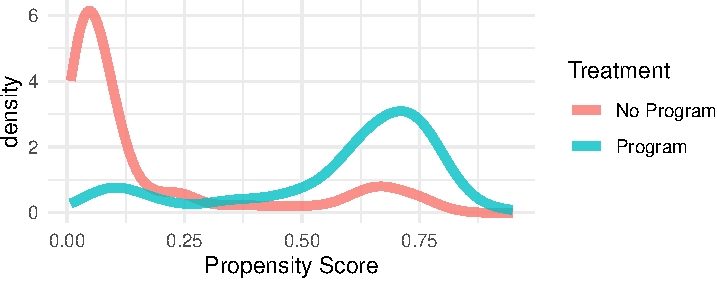
\includegraphics{soo_matching_files/figure-beamer/unnamed-chunk-11-1} \end{center}

\end{frame}

\begin{frame}[fragile]

Matching on the PS.

\begin{Shaded}
\begin{Highlighting}[]
\NormalTok{match_pscore <-}\StringTok{ }\KeywordTok{Match}\NormalTok{(}\DataTypeTok{Y =}\NormalTok{ lalonde}\OperatorTok{$}\NormalTok{re78, }
                      \DataTypeTok{Tr =}\NormalTok{ lalonde}\OperatorTok{$}\NormalTok{treat, }
                      \DataTypeTok{X =}\NormalTok{ ps_model}\OperatorTok{$}\NormalTok{fitted.values)}
\CommentTok{#summary(match_pscore)}
\end{Highlighting}
\end{Shaded}

\begin{center}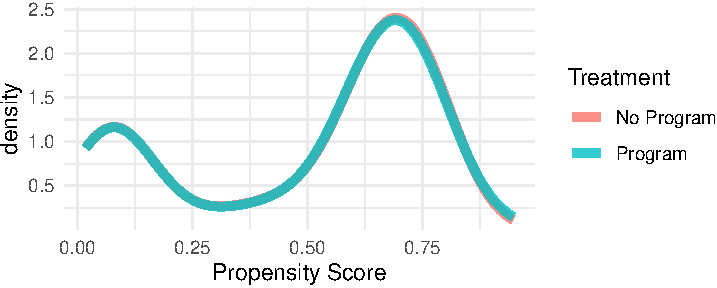
\includegraphics{soo_matching_files/figure-beamer/unnamed-chunk-13-1} \end{center}

\end{frame}

\begin{frame}

\begin{table}[ht]
\centering
\caption{Covariate Balance in Propensity Score Matched Data} 
\label{tab:pscore-bal}
\scalebox{0.75}{
\begin{tabular}{rrrrrrrr}
  \hline
 & mean.Tr & mean.Co & sdiff & sdiff.pooled & var.ratio & T pval & KS pval \\ 
  \hline
age & 25.82 & 24.51 & 18.28 & 18.28 & 0.44 & 0.18 & 0.00 \\ 
  educ & 10.35 & 10.48 & -6.79 & -6.79 & 0.63 & 0.55 & 0.09 \\ 
  black & 0.84 & 0.85 & -2.97 & -2.97 & 1.06 & 0.32 &  \\ 
  hispan & 0.06 & 0.03 & 10.42 & 10.42 & 1.67 & 0.16 &  \\ 
  married & 0.71 & 0.65 & 12.74 & 12.74 & 0.91 & 0.23 &  \\ 
  nodegree & 0.19 & 0.22 & -6.88 & -6.88 & 0.91 & 0.42 &  \\ 
  re74 & 2095.57 & 2100.16 & -0.09 & -0.09 & 1.58 & 0.99 & 0.00 \\ 
  re75 & 1532.06 & 1920.09 & -12.05 & -12.05 & 1.00 & 0.24 & 0.00 \\ 
  re78 & 6349.14 & 7035.08 & -8.72 & -8.72 & 1.19 & 0.33 & 0.00 \\ 
   \hline
\end{tabular}
}
\end{table}

\begin{itemize}
\tightlist
\item
  How does this compare to our previous approach to matching?
\end{itemize}

\end{frame}

\begin{frame}{Weighting}

\begin{itemize}
\item
  Idea: weight each observation in the control group such that it looks
  like the treatment group (i.e., good covariate balance)\footnote<.->{Matching
    is a special case of weighting!}
\item
  Suppose, there are two types of cats, each with a different
  probability of receiving treatment \(D\). In this example, we can
  assign the lone cats in the off-diagonal cells a weight of 3.
\end{itemize}

\begin{center}
 \begin{tabular}{||c c c ||} 
 \hline
 & P(D = 1) = 0.75 & P(D = 1) = 0.25\\ [0.5ex] 
 \hline\hline
 D = 1 & \includegraphics[scale=0.10]{smiley_cat1} \includegraphics[scale=0.10]{smiley_cat1} \includegraphics[scale=0.10]{smiley_cat1} &  \includegraphics[scale=0.30]{smiley_cat2}\\ 
 \hline
 D = 0 & \includegraphics[scale=0.30]{crying_cat1} & \includegraphics[scale=0.10]{crying_cat2} \includegraphics[scale=0.10]{crying_cat2} \includegraphics[scale=0.10]{crying_cat2}\\
 \hline
\end{tabular}
\end{center}

\end{frame}

\begin{frame}{Inverse Probability Weighting (IPW)}

Weighting on the Propensity Score \(\pi(X_i)\)

\[\tau_{ATE} = \mathbb{E}\Big[Y_i \cdot \frac{D_i - \hat{\pi}(X_i) }{\hat{\pi}(X_i)\cdot[1-\hat{\pi}(X_i)]}\Big]\]

The sample analog is (\(\hat{\tau}_{ATE}\)):

\[\frac{1}{N} \sum_{i=1}^{N} \Big\{ Y_i \cdot \frac{D_i - \hat{\pi}(X_i) }{\hat{\pi}(X_i)\cdot[1-\hat{\pi}(X_i)]}  \Big\} = \frac{1}{N} \sum_{i=1}^{N} \Big\{ \frac{D_i \cdot Y_i }{\hat{\pi}(X_i)} \Big\} -  \frac{1}{N} \sum_{i=1}^{N} \Big\{ \frac{(1 - D_i) \cdot Y_i}{[1-\hat{\pi}(X_i)]}  \Big\}\]

\end{frame}

\begin{frame}{Inverse Probability Weighting (IPW)}

\[\tau_{ATT} = \mathbb{E}\Big[Y_i \cdot \frac{D_i - \hat{\pi}(X_i) }{1-\hat{\pi}(X_i)}\Big] \cdot \mathbb{P}(D_i =1)^{-1}\]

With sample analog:

\[\hat{\tau}_{ATT} = \dfrac{1}{N_1} \sum_{i=1}^{N} \Big\{ Y_i \cdot \frac{D_i - \hat{\pi}(X_i) }{1-\hat{\pi}(X_i)}  \Big\}\]

\end{frame}

\section{Additional Notes}\label{additional-notes}

\end{document}
